
\RequirePackage{algorithmic}


\documentclass{beamer}

\usepackage[utf8x]{inputenc}
\usepackage{default}
\usepackage{ beamerthemesplit}



\title{Robot Localization Simulator}
\author{ Prateek Garg, Kumar Ashwani, Apurv Verma }
\date {\today}

\begin{document}
\frame{\titlepage}

\frame
{
  \frametitle{Acknowledgement}
We would like to acknowledege Assistant Professor Apurva Mudgal for helping us understand the difficult Robot Localization Algorithm.
 His supervision made it appear all very easy.
 We are also thankful to the ever enthusiastic CGAL community for helping us with the various CGAL issues.


}

\frame
{
  \frametitle{Introduction}

A robot is placed at an unknown point inside a simple polygon $ P $. The robot has a map of 
$ P$ and can compute visibility polygon from its current location. The robot must determine its correct 
location inside the polygon $P $ at a minimum cost of travel distance.

}


\frame[allowframebreaks]
{
  \frametitle{Robot Localization Algorithm}


{\bf Input:}\\
Map polygon $P$, the visibility polygon $V$.
\\
{\bf Output:}\\
The robot localizes to its actual position $h \in H$
\\
\begin{algorithmic}[1]
  \STATE Compute the set of hypotheses $H$.
 \WHILE{ $ | H | > 1$ } 
  \STATE Compute the majority-rule map $P_{maj}$
  \STATE Compute the polygons $G_{ij}$ for each pair of hypotheses, $h_{i}$ and $h_{j}$
  \STATE Compute the majority rule map $K_{i}$ of $G_{ij}$'s
  \STATE Find the edges on the boundary of $K_{i}$ which are not on the boundary of $P_{maj}$
  \STATE Draw grids and compute the set of coordinates $Q_{H}$ on these edges.
  \STATE Make instance $I_{P,H}$  of $\frac{1}{2}$ -Group Steiner Problem
  \STATE Solve $I_{P,H}$ to compute a half computing path $C \subset P_{maj}$
  \STATE Half-Localize by tracing $C $ and making observations at coordinates $Q_{H}$
  \STATE Move back to the starting location.
 \ENDWHILE
\end{algorithmic}
}

\frame
{
  \frametitle{Geometrical Algorithms}

Visibility polygon is an indispensable component in the hypothesis generation step of the algorithm. Since CGAL had no inbuilt support
 for computing visibility polygons we implemented the following two routines for our purposes.
\begin{itemize}
 \item Visibility Polygon of a point inside a polygon
 \item Visibility Polygon of an edge of the polygon.
\end{itemize}

}

\frame[allowframebreaks]
{
\frametitle{Visibility Polygon of a Point Inside a Polygon}
\begin{definition}
 {\bf Visibility Polygon of Point:} $p$ is the bounded polygonal region of all points of the polygon visible from $p$.  
\end{definition}

}

\frame
{

{\bf Algorithm}
\frametitle{Algorithm}

\begin{enumerate}
 \item 
Collect all the vertices of the polygon which are visible from the point $P$.
\item
Iterate over the list of visible vertices and for each reflex vertex, compute the spurious vertex introduced in the visibility polygon.
\item
Finally sort all the vertices in an order so that they form a simple polygon.
\end{enumerate}

}

\frame[allowframebreaks]
{
\frametitle{Examples}

\begin{figure}[h]
\begin{center}
\scalebox{0.30}{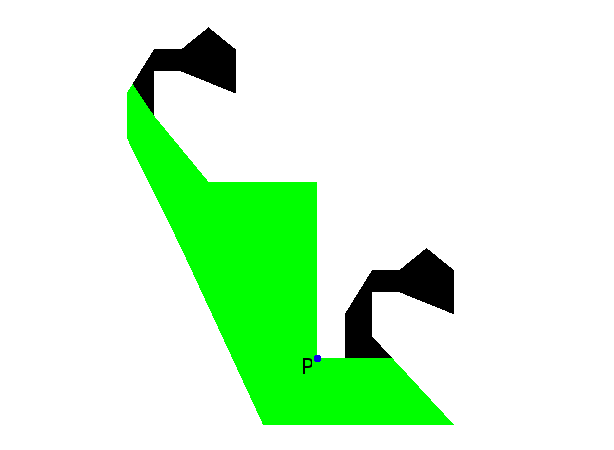
\includegraphics{Images/VisibilityPolygonBird.png}}
\caption{\label{fig:Visibility Polygon of Point}Visibility Polygon of Point}
\end{center}
\end{figure}


\begin{figure}[h]
\begin{center}
\scalebox{0.40}{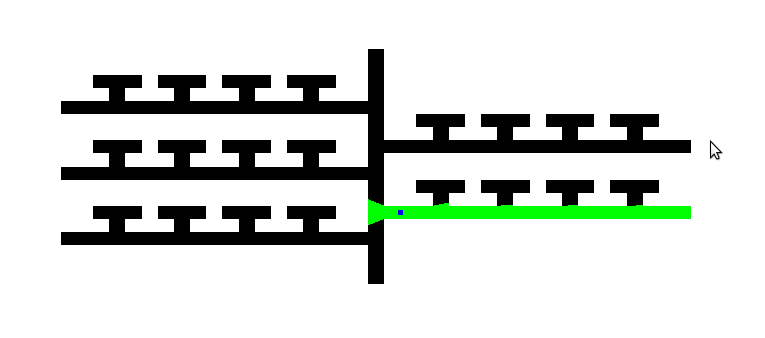
\includegraphics{Images/VisibilityPointOffice.png}}
\caption{\label{fig:Visibility Polygon of Point}Visibility Polygon of Point}
\end{center}
\end{figure}

}

\frame
{
\frametitle{Visibility Polygon of an edge of the polygon}

\begin{definition}
 {\bf Visibility Polygon of Edge:} $e$ is the bounded polygonal region of all points of the polygon visible from any point on the edge $e$. 
\end{definition}

The algorithm for the visibility polygon of an edge has been taken from \cite{key3}.
}

\frame
{
\frametitle{Visibility Polygon of an edge of the polygon}
\begin{figure}[h]
\begin{center}
\scalebox{0.30}{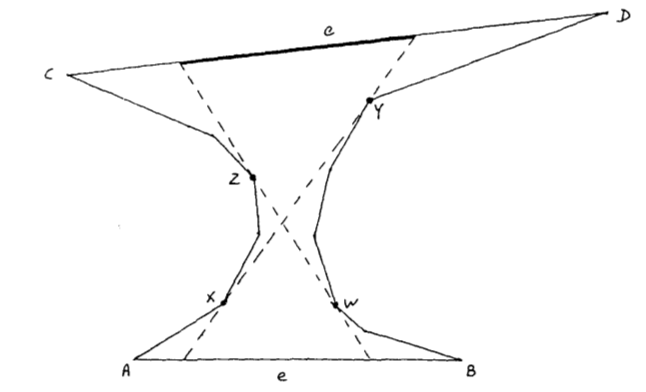
\includegraphics{Images/Cusp.png}}
\caption{\label{fig:Visibility Polygon of Edge}Visibility Polygon of Edge, Illustration taken from:\cite{key3}}
\end{center}
\end{figure}

}

\frame[allowframebreaks]
{
\frametitle{Algorithm}
\begin{enumerate}
\item
Compute the shortest path $P_{AC}$, from A to C and the shortest path $P_{BD}$, from B to D. Call this pair 1.
\item
Similarly compute the shortest path  $P_{AD}$, from A to D and the shortest path  $P_{BC}$,  from B to C. Call this pair 2.
\item
Find out which of these pairs is outward convex. An outward convex pair implies an hourglass shape is formed by the two paths.
\item
If none of the pairs is outward convex this means that no portion of edge $CD$ is visible from any point on edge $AB$ and we can 
completely ignore such an edge.
\item
If one of the pairs is outward convex then without loss of generality, let pair 1 be the outward convex pair. Now compute the shortest 
paths  $P_{AD}$ and  $P_{BC}$.
\item
Let $X$ be the point where path $P_{AD}$ and $P_{AC}$ split and let  $W$ be the point where path $P_{BD}$ and $P_{BC}$ split. Let $Y$ be
the next point on the path  $P_{AD}$ and $Z$ be the next point on the path   $P_{BC}$. Extending $XY$ we get one extreme point of the 
portion of $CD$ visible from $AB$. We repeat this on other side to get the other extreme point.


\end{enumerate}

}

\frame[allowframebreaks]
{
\frametitle{Shortest Path Calculation}
For the calculation of shortest path between any two vertices of the polygon the following property was exploited.
\begin{itemize}
 \item The shortest path must turn only at vertices of the polygon.
 \item It is possible to move from one vertex to the another only if they are visible to each other.
\end{itemize}
}

\frame[allowframebreaks]
{
\frametitle{Visibility Graph}
\begin{definition}
{\bf Visibility Graph}The visibility graph of a polygon can be formed as follows. Draw a vertex corresponding to each vertex in the 
polygon. Draw an edge between two vertices if the line joining the corresponding vertices in the polygon lies completely inside the 
polygon.
\end{definition}


\begin{figure}
\begin{center}
\scalebox{0.4}{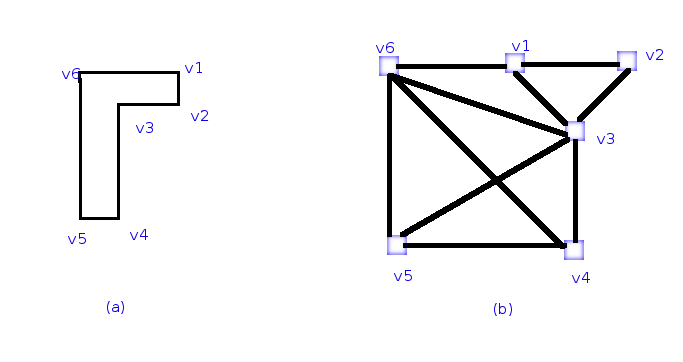
\includegraphics{Images/visibilitygraph.png}}
\caption{\label{fig:Construction} Visibility Graph}
\end{center}
\end{figure}
}

\frame
{
\frametitle{Examples}

\begin{figure}
\begin{center}
\scalebox{0.30}{
\includegraphics{Images/VisibilityLine1.png}}
\caption{\label{fig:Visibility Polygon of Edge}Visibility Polygon of Edge}
\end{center}
\end{figure}

}

\frame
{
\frametitle{Examples}
\begin{figure}
\begin{center}
\scalebox{0.30}{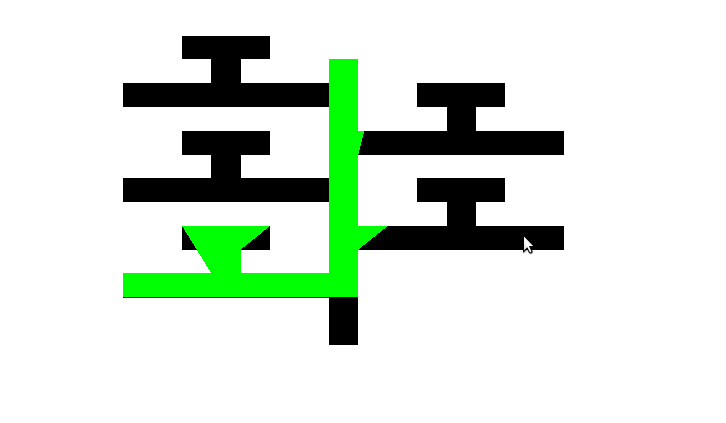
\includegraphics{Images/VisibilityLine2.png}}
\caption{\label{fig:Visibility Polygon of Edge}Visibility Polygon of Edge}
\end{center}
\end{figure}

}


\frame
{
 \frametitle{Hypothesis Generation}

\begin{theorem}
 A point, $P$ inside a simple polygon sees atleast one edge of the polygon completely.
\end{theorem}

\begin{definition}
 {\bf Spurious Edge:} In the visibility polygon of a point, an edge is called a spurious edge if it is obtained by extending the line
 joining the point $P$ and a reflex vertex till it meets the polygon.
\end{definition}


\begin{theorem}
 The visibility polygon of a point $P$ has atleast one edge which completely overlaps with an edge of the original polygon.
\end{theorem}

}


\frame
{
\frametitle{Algorithm}
\begin{enumerate}
 \item Iterate over the edges of the polygon and the edges of the map. and find an edge in the map which has the same length and
 orientation as an edge in the polygon.

 \item
 Translate the visibility polygon such that the matching edge of the map polygon
and the visibility polygon coincide.

 \item
 For each of the remaining edges of the visibility polygon, check whether a 
complete match exists or not. If all the remaining edges match, the point where the
origin was translated is added to the set of hypotheses.

\end{enumerate}

}

\frame[allowframebreaks]
{
\frametitle{Examples}

\begin{figure}
\begin{center}
\scalebox{0.40}{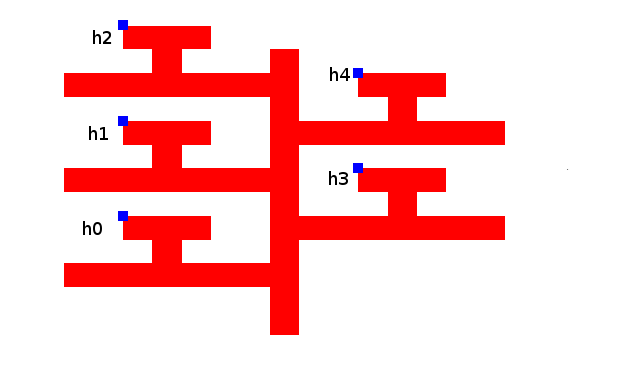
\includegraphics{Images/Hypothesis_office.png}}
\caption{\label{fig:Hypothesis Generation}Hypothesis Generation}
\end{center}
\end{figure}


\begin{figure}
\begin{center}
\scalebox{0.40}{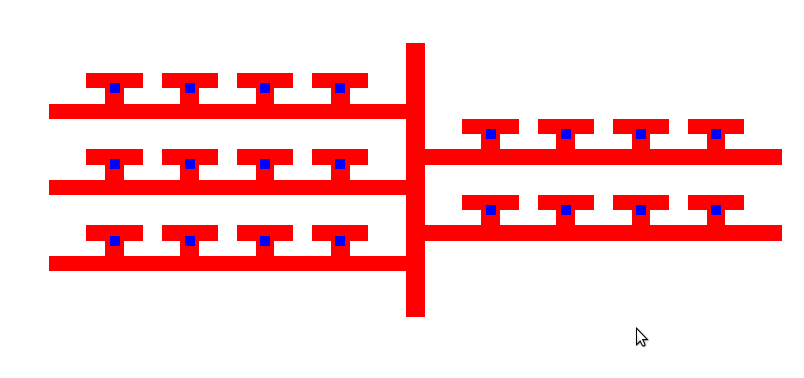
\includegraphics{Images/HypothesisOfficeAnti.png}}
\caption{\label{fig:Hypothesis Generation}Hypothesis Generation}
\end{center}
\end{figure}

}

\frame
{
\frametitle{Majority Rule Map}

The following example taken from \cite{key1} demonstrates the construction of a majority rule map.

\begin{figure}[h]
\begin{center}
\scalebox{0.50}{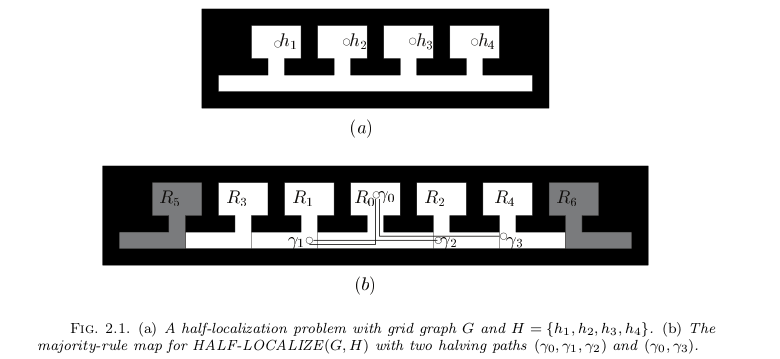
\includegraphics{Images/MajorityMapExample.png}}
\caption{\label{fig:Construction}Majority Rule Map Construction}
\end{center}
\end{figure}
}

\frame
{
\frametitle{Majority Rule Map}

${h_{1},h_{2},h_{3},h_{4}}$ form the set of hypotheses. Arbitrarily we choose $h_{1}$ as the origin. Next we translate all the 
remaining hypotheses to $h_{1}$ to obtain the overlay arrangement. The overlay arrangement contains the following faces
$R_{0},R_{1},R_{2},R_{3},R_{4},R_{5},R_{6}$. Recall from the definition of $Maj(\gamma)$



$  Maj(R_{0})  =  {h_{1}, h_{2}, h_{3}, h_{4}} $ , $  Maj(R_{1})  =  { h_{2}, h_{3}, h_{4}} $, $ Maj(R_{2})  =  {h_{1}, h_{2}, h_{3}} $,
$  Maj(R_{3})  =  {h_{3}, h_{4}} $ and $  Maj(R_{4})  =  {h_{1}, h_{2}} $



In the majority rule map the region $R_{5}$ and $R_{6}$ are blocked because less than half the hypothesis said that they were
 traversable. They have been shown in gray.

}
\end{document}
